\documentclass[aspectratio=169]{beamer}

\usepackage[T1]{fontenc}
\usepackage[brazil]{babel}
\usepackage[utf8]{inputenc}
\usepackage{graphicx}

\newcommand{\inframe}[2]{
    \begin{frame}{#1}
        #2
    \end{frame}
}

\newcommand{\intwocols}[2]{
    \begin{columns}
        \begin{column}{0.5\textwidth}
            #1
        \end{column}
        \begin{column}{0.5\textwidth}
            #2
        \end{column}
    \end{columns}
}


\newcommand{\ttwocframe}[3]{
    \inframe{#1}{\intwocols{#2}{#3}}
}

\newcommand{\twocframe}[2]{
    \inframe{}{#1}{#2}
}
% Choose the Inf theme
\usetheme{Inf}

% Define the title with \title[short title]{long title}
\title[Trabalho 1 - OpenMP]
      {OpenMP - Simulação de N Corpos}

% Optional subtitle
\subtitle{INF01008 - Programação Paralela}

\date{Setembro de 2026}

% Author information
\author{Lucas Timm}
\institute{Instituto de Informática | Escola de Engenharia --- UFRGS }

\begin{document}

\InfTitlePage

\section{Detalhes}

\frame{
    \frametitle{Introdução}
    \intwocols{
      \begin{enumerate}
	\item Duas famílias de algoritmo: Força Bruta e Barnes-Hutt.
	\item Força bruta : O(n²)
	\item Barnes-Hutt : O(nlog(n))
	\item Força bruta mostra mais potencial para o estudo de  paralelização.
	\item Cada thread realiza uma quantidade similar de computação.
      \end{enumerate}
    }{
      $$\vec F = \frac{\vec r}{\|\mathbf{r}\|^3}$$
      $$S = S_0 + V_0 t + \frac{at^2}{2}$$
    }
}


\frame{
  \frametitle{Ambiente}
  \intwocols{
    \begin{itemize}
      \item Ambiente computacional PCAD
      \item Nó hype5
      \item CPU: 2 x Intel(R) Xeon(R) E5-2650 v3, 2.3 GHz, 40 threads, 20 cores
      \item RAM: 128 GB DDR4
      \item MB: HP ProLiant XL190r Gen9
    \end{itemize}
  }
  {
    \begin{figure}
      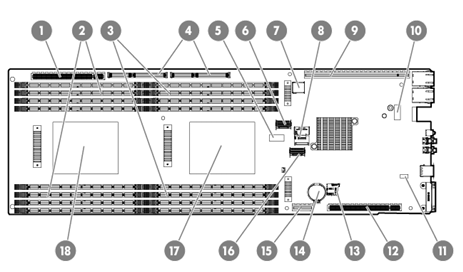
\includegraphics[width=\linewidth]{placa_mae.png}
      \caption{Esquemática HPE ProLiant XL190r Gen9 Server}
    \end{figure}
  }
}

\section{Metodologia}

\frame{
    \frametitle{Implementação}

    \intwocols{
      \begin{enumerate}
	\item Implementação em C++
	  \begin{itemize}
	    \item -std=c++23 -O3 -march=native -ffast-math -fopenmp 
	    \item Input: .csv com N coordenadas 3d
	    \item Output: "S/P;Corpos;Threads;Tempo"
	  \end{itemize}
	\item Valores de entrada aleatórios, gerados em Python
	\item Experimento realizado em script bash, alterando threads e entrada
	\item Processamento de resultados em Python
      \end{enumerate}
    }{
    \begin{figure}
      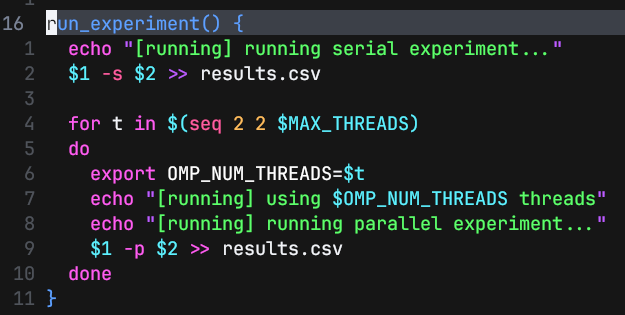
\includegraphics[width=\linewidth]{bash_run.png}
      \caption{Principal função no script bash}
    \end{figure}
    }
}

\frame{
    \frametitle{Algoritmos}

    \intwocols
    {
      Simulação Serial:
      \begin{enumerate}
	\item omp simd
	\begin{itemize}
	  \item Ler corpo $i$
	  \item Ler outros corpos, $j$
	  \item Calcular participação $\vec F_{ij}$
	  \item Incrementar na força do corpo $i$
	  \item Reduzir na força do corpo $j$
	\end{itemize}
	\item omp simd
	\begin{itemize}
	  \item Ler corpo $i$
	  \item Atualizar velocidade e posição $i$
	\end{itemize}
      \end{enumerate}
    }
    {
      Simulação Paralela:
      \begin{enumerate}
	\item omp for
	\begin{itemize}
	  \item Ler corpo $i$
	  \item Ler outros corpos, $j$
	  \item Calcular participação $\vec F_{ij}$
	  \item Incrementar na força do corpo $i$
	\end{itemize}
	\item omp barrier
	\item omp for simd
	\begin{itemize}
	  \item Ler corpo $i$
	  \item Atualizar velocidade e posição $i$
	\end{itemize}
      \end{enumerate}
    }
}

\section{Resultados}

\frame{
    \frametitle{Escalabilidade Serial}

    \intwocols{
      \begin{figure}
        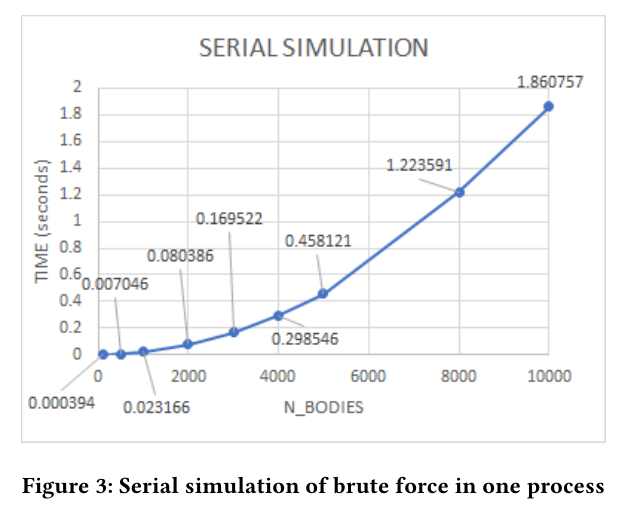
\includegraphics[width=\linewidth]{chen.png}
        \caption{Número de Corpos vs Tempo de Execução, Jiayu Chen 2021}
      \end{figure}
    }{
      \begin{figure}
        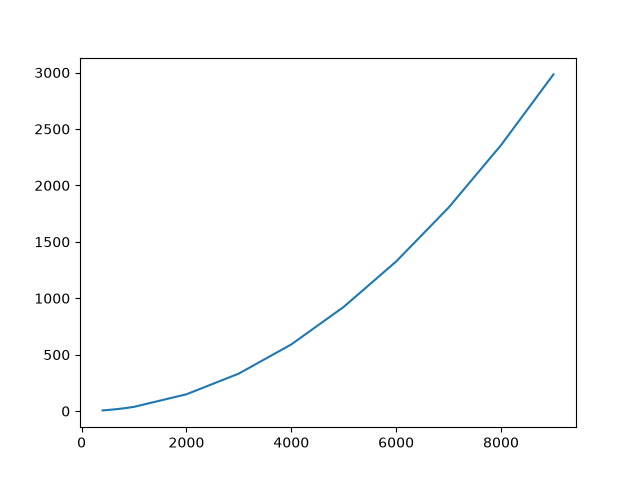
\includegraphics[width=\linewidth]{serial_time.png}
        \caption{Número de Corpos vs Tempo de Execução}
      \end{figure}
    }
}

\frame{
      \frametitle{Threads por Tempo de Execução, Série Completa}
      \begin{figure}
	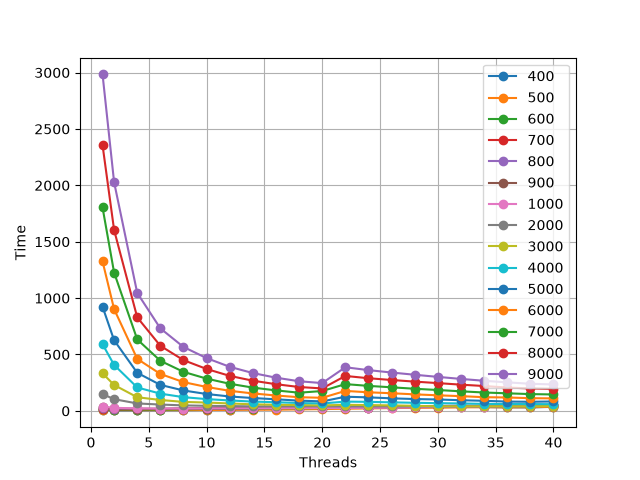
\includegraphics[width=275pt]{threads_time.png}
      \end{figure}
}

\frame{
      \frametitle{Threads por Speedup, Série Completa}
      \begin{figure}
      	  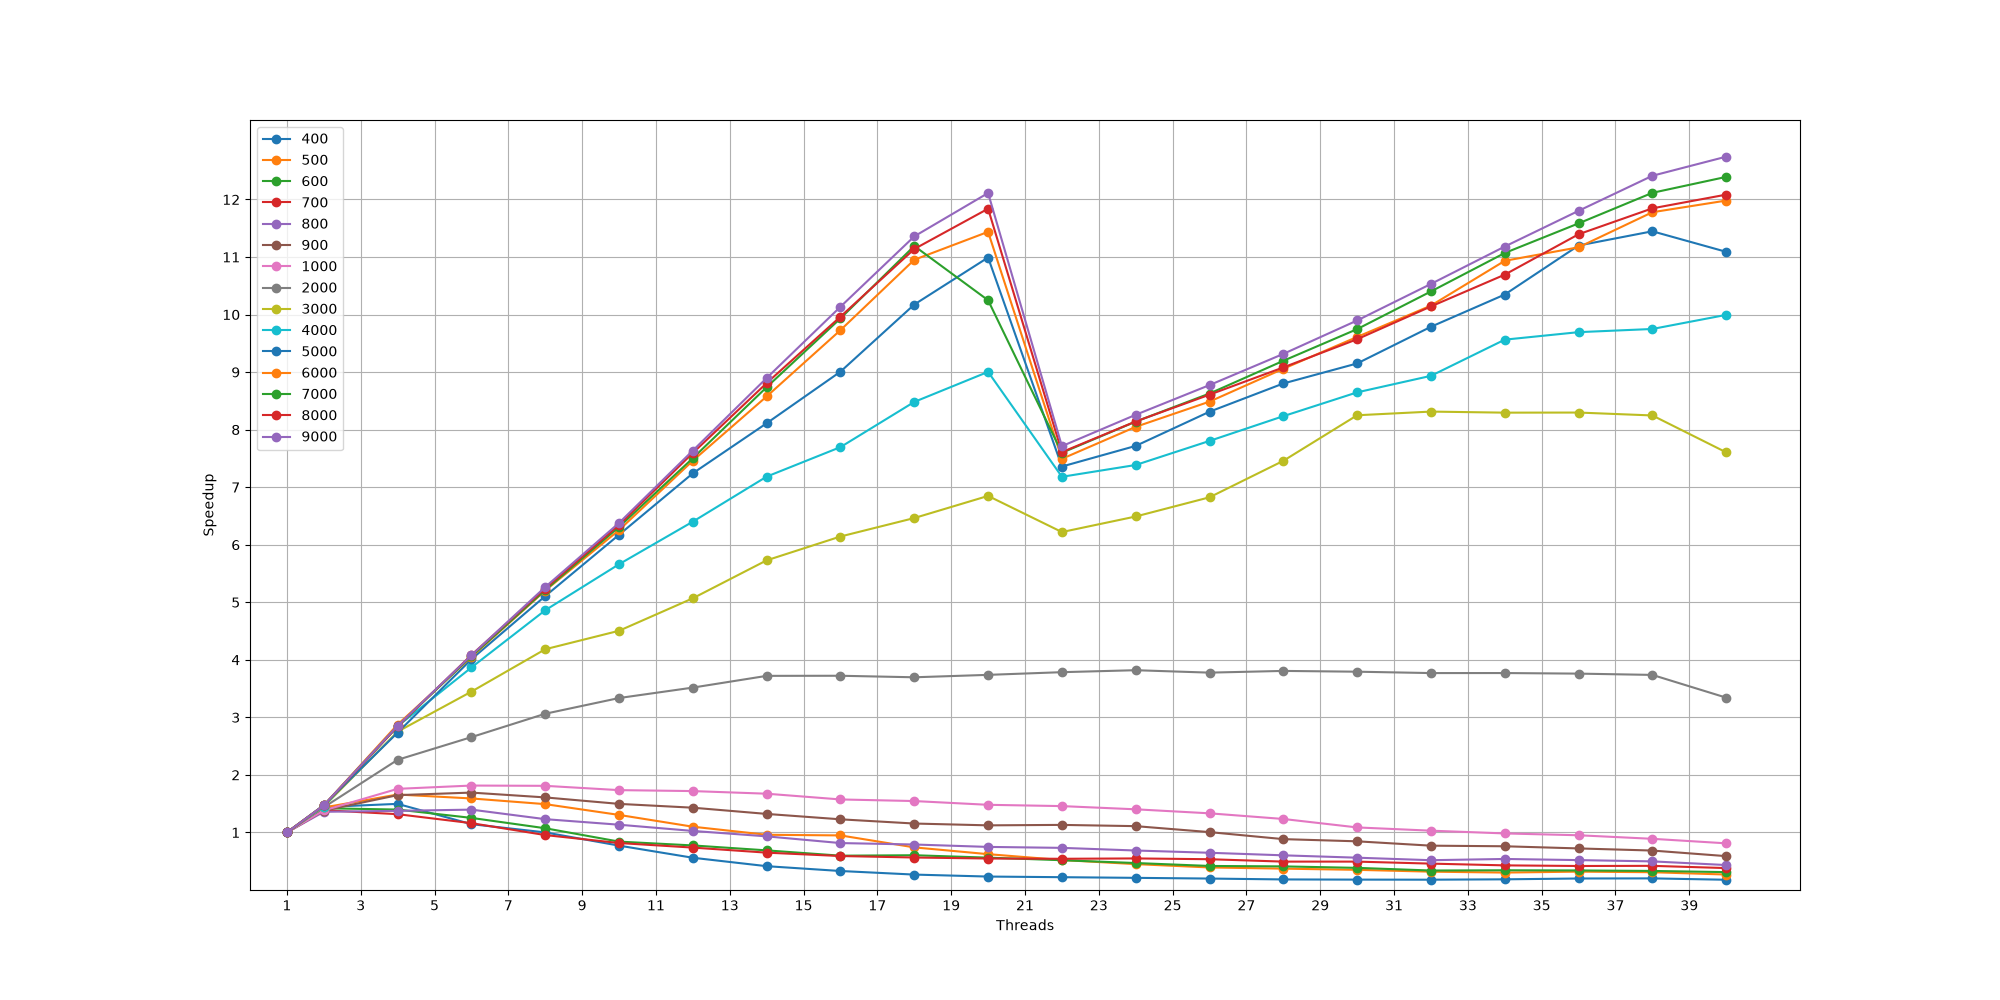
\includegraphics[width=400pt]{threads_speedup.png}
      \end{figure}
}


\frame{
      \frametitle{Mapa de Calor, Speedup}
      \begin{figure}
      	  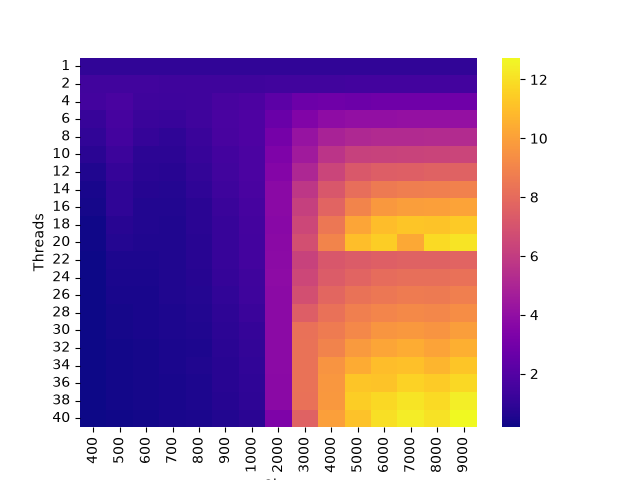
\includegraphics[width=260pt]{heatmap_speedup.png}
      \end{figure}
}

\section*{}

\begin{frame}
    \frametitle{Obrigado!}
    \InfContacts
\end{frame}

\end{document}
